\documentclass[tikz,border=3pt]{standalone}

\usepackage[T1]{fontenc}
\usepackage{sourcesanspro}
\usepackage{amsmath}
\usepackage{amssymb}
\usetikzlibrary{arrows.meta,calc,positioning}

\definecolor{ink}{HTML}{182033}
\definecolor{muted}{HTML}{64748B}
\definecolor{plane}{HTML}{FBFCFE}
\definecolor{planeedge}{HTML}{CBD5E1}
\definecolor{qwen}{HTML}{2563EB}
\definecolor{gemma}{HTML}{D97706}
\definecolor{ministral}{HTML}{7C3AED}
\definecolor{graph}{HTML}{0F766E}
\definecolor{success}{HTML}{15803D}

\tikzset{
  >=Latex,
  every node/.style={
    font=\sffamily\fontsize{7.4}{8.5}\selectfont,
    text=ink,
    align=center
  },
  stage/.style={
    font=\sffamily\bfseries\fontsize{8.8}{10.0}\selectfont,
    text=ink
  },
  model/.style={
    rounded corners=0.8mm,
    minimum width=42mm,
    minimum height=10.5mm,
    inner sep=1.5mm,
    fill=white,
    line width=0.7pt
  },
  event/.style={
    rounded corners=0.8mm,
    minimum width=31mm,
    minimum height=12mm,
    inner sep=1.3mm,
    fill=white,
    line width=0.75pt,
    font=\sffamily\bfseries\fontsize{6.7}{7.6}\selectfont
  },
  component/.style={
    rounded corners=0.8mm,
    minimum width=37mm,
    minimum height=15mm,
    inner sep=1.3mm,
    fill=white,
    draw=graph,
    line width=0.8pt
  },
  decision/.style={
    rounded corners=1.4mm,
    minimum width=31mm,
    minimum height=12mm,
    inner sep=1.5mm,
    fill=white,
    draw=ink,
    line width=0.9pt,
    font=\sffamily\bfseries\fontsize{7.2}{8.2}\selectfont
  },
  flow/.style={
    -{Latex[length=1.7mm,width=1.2mm]},
    line width=0.8pt
  },
  support/.style={
    -{Latex[length=1.5mm,width=1.05mm]},
    draw=graph,
    line width=0.75pt
  }
}

\begin{document}
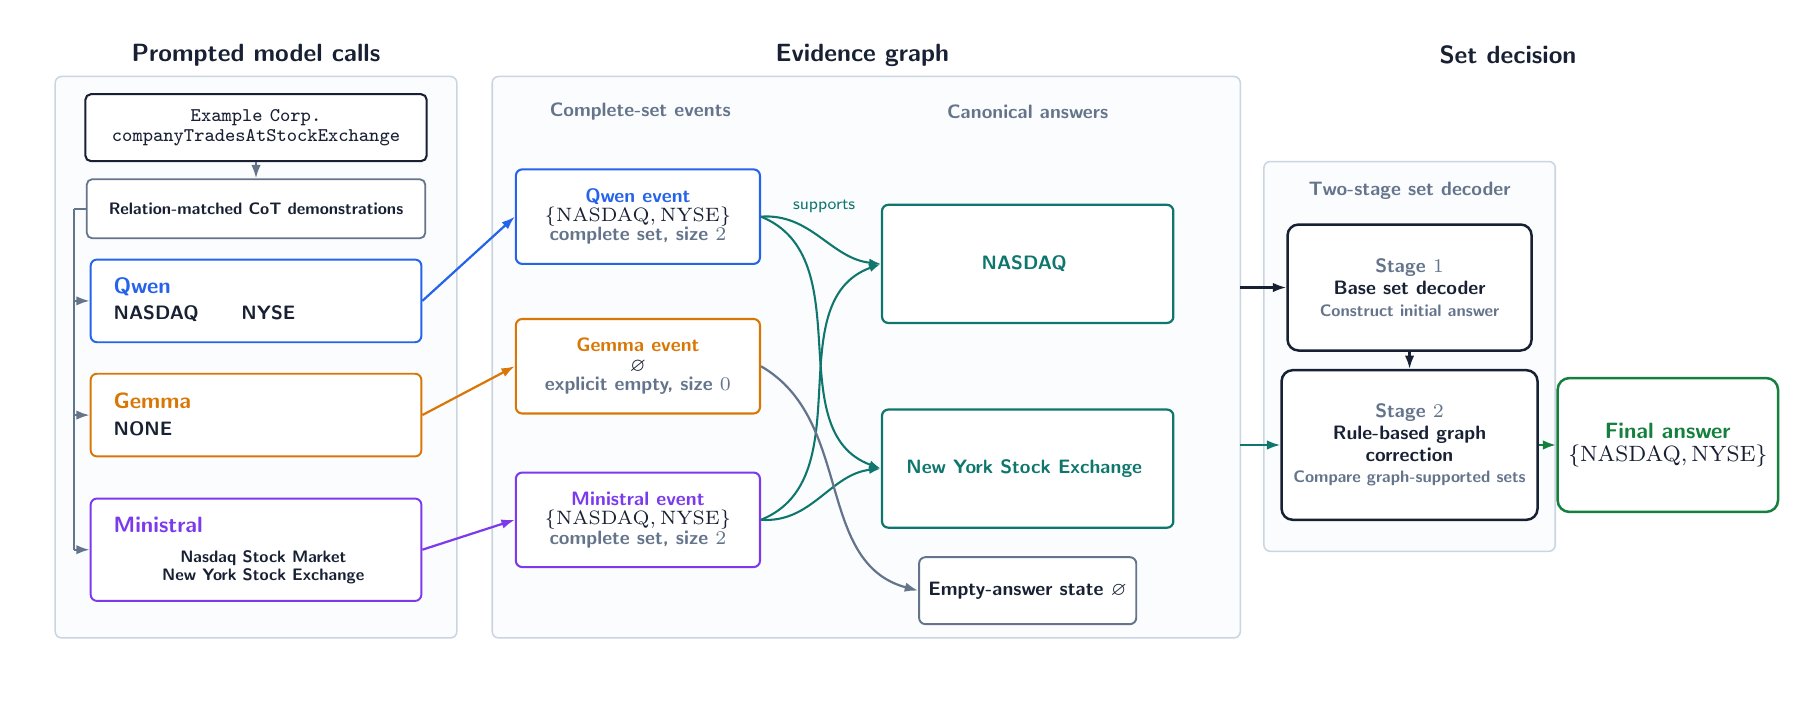
\begin{tikzpicture}[x=1cm,y=1cm]

\path[fill=white] (-0.15,-0.15) rectangle (22.15,8.35);

\node[stage] at (2.75,8.00) {Prompted model calls};
\node[stage] at (10.45,8.00) {Evidence graph};
\node[stage] at (18.65,8.00) {Set decision};

% ---------------------------------------------------------------------------
% Prompted independent model calls
% ---------------------------------------------------------------------------
\path[fill=plane,draw=planeedge,line width=0.55pt,rounded corners=0.8mm]
  (0.20,0.60) rectangle (5.30,7.73);

\node[
  rounded corners=0.7mm,
  draw=ink,
  fill=white,
  line width=0.75pt,
  minimum width=43mm,
  minimum height=8.5mm,
  text width=41mm,
  font=\sffamily\bfseries\fontsize{6.8}{7.8}\selectfont
] (query) at (2.75,7.08) {
  \texttt{Example Corp.}\\[-0.1mm]
  \texttt{companyTradesAtStockExchange}
};

\node[
  rounded corners=0.7mm,
  draw=muted,
  fill=white,
  line width=0.65pt,
  minimum width=43mm,
  minimum height=7.5mm,
  font=\sffamily\bfseries\fontsize{6.5}{7.4}\selectfont
] (demos) at (2.75,6.05) {Relation-matched CoT demonstrations};

\node[model,draw=qwen] (qwenbox) at (2.75,4.88) {};
\node[
  anchor=north west,
  text=qwen,
  font=\sffamily\bfseries\fontsize{8}{9}\selectfont
] at ($(qwenbox.north west)+(1.8mm,-1.3mm)$) {Qwen};
\node[
  anchor=south west,
  text=ink,
  font=\sffamily\bfseries\fontsize{6.7}{7.5}\selectfont
] at ($(qwenbox.south west)+(1.8mm,1.5mm)$) {NASDAQ\qquad NYSE};

\node[model,draw=gemma] (gemmabox) at (2.75,3.43) {};
\node[
  anchor=north west,
  text=gemma,
  font=\sffamily\bfseries\fontsize{8}{9}\selectfont
] at ($(gemmabox.north west)+(1.8mm,-1.3mm)$) {Gemma};
\node[
  anchor=south west,
  text=ink,
  font=\sffamily\bfseries\fontsize{6.7}{7.5}\selectfont
] at ($(gemmabox.south west)+(1.8mm,1.5mm)$) {NONE};

\node[model,draw=ministral,minimum height=13mm] (ministralbox) at (2.75,1.72) {};
\node[
  anchor=north west,
  text=ministral,
  font=\sffamily\bfseries\fontsize{8}{9}\selectfont
] at ($(ministralbox.north west)+(1.8mm,-1.3mm)$) {Ministral};
\node[
  anchor=south west,
  text=ink,
  text width=38mm,
  font=\sffamily\bfseries\fontsize{6.2}{7.0}\selectfont
] at ($(ministralbox.south west)+(1.8mm,1.0mm)$) {
  Nasdaq Stock Market\\[-0.1mm]New York Stock Exchange
};

% The query and demonstrations are shared prompt context.  The three calls
% are independent; vertical placement must not imply model-to-model flow.
\draw[flow,draw=muted] (query.south) -- (demos.north);
\draw[draw=muted,line width=0.65pt] (demos.west) -- (0.44,6.05);
\draw[draw=muted,line width=0.65pt] (0.44,6.05) -- (0.44,1.72);
\draw[flow,draw=muted] (0.44,4.88) -- (qwenbox.west);
\draw[flow,draw=muted] (0.44,3.43) -- (gemmabox.west);
\draw[flow,draw=muted] (0.44,1.72) -- (ministralbox.west);

% ---------------------------------------------------------------------------
% Evidence graph: complete-set evidence events and canonical components
% ---------------------------------------------------------------------------
\path[fill=plane,draw=planeedge,line width=0.55pt,rounded corners=0.8mm]
  (5.75,0.60) rectangle (15.25,7.73);

\node[
  text=muted,
  font=\sffamily\bfseries\fontsize{7.1}{8.1}\selectfont
] at (7.63,7.28) {Complete-set events};
\node[
  text=muted,
  font=\sffamily\bfseries\fontsize{7.1}{8.1}\selectfont
] at (12.55,7.28) {Canonical answers};

\node[event,draw=qwen] (qevent) at (7.60,5.95) {
  \textcolor{qwen}{Qwen event}\\[-0.2mm]
  \(\{\mathrm{NASDAQ},\mathrm{NYSE}\}\)\\[-0.2mm]
  \textcolor{muted}{complete set, size \(2\)}
};

\node[event,draw=gemma] (gevent) at (7.60,4.05) {
  \textcolor{gemma}{Gemma event}\\[-0.2mm]
  \(\varnothing\)\\[-0.2mm]
  \textcolor{muted}{explicit empty, size \(0\)}
};

\node[event,draw=ministral] (mevent) at (7.60,2.10) {
  \textcolor{ministral}{Ministral event}\\[-0.2mm]
  \(\{\mathrm{NASDAQ},\mathrm{NYSE}\}\)\\[-0.2mm]
  \textcolor{muted}{complete set, size \(2\)}
};

\node[component] (nasdaq) at (12.55,5.35) {
  \textcolor{graph}{\textbf{NASDAQ}}
};

\node[component] (nyse) at (12.55,2.75) {
  \textcolor{graph}{\textbf{New York Stock Exchange}}
};

\node[
  rounded corners=0.8mm,
  minimum width=25mm,
  minimum height=8.5mm,
  fill=white,
  draw=muted,
  line width=0.7pt,
  font=\sffamily\bfseries\fontsize{6.6}{7.5}\selectfont
] (emptystate) at (12.55,1.20) {Empty-answer state \(\varnothing\)};

% One arrow per exact event-component membership.  Curves keep the two
% complete sets visually intact without implying candidate-wise generation.
\draw[support] (qevent.east) to[out=4,in=174] node[pos=0.53,above=2.0mm,
  font=\sffamily\fontsize{6.1}{7.0}\selectfont,text=graph] {supports} (nasdaq.west);
\draw[support] (qevent.east) to[out=-22,in=160] (nyse.west);
\draw[support] (mevent.east) to[out=22,in=200] (nasdaq.west);
\draw[support] (mevent.east) to[out=-4,in=186] (nyse.west);
\draw[flow,draw=muted] (gevent.east) to[out=-30,in=165] (emptystate.west);

% Model outputs become event nodes; same-family sample multiplicities are
% omitted in this illustrative row to keep the graph readable.
\draw[flow,draw=qwen] (qwenbox.east) -- (qevent.west);
\draw[flow,draw=gemma] (gemmabox.east) -- (gevent.west);
\draw[flow,draw=ministral] (ministralbox.east) -- (mevent.west);

% ---------------------------------------------------------------------------
% Set decision: both operations belong to one two-stage decoder.
% ---------------------------------------------------------------------------
\path[fill=plane,draw=planeedge,line width=0.55pt,rounded corners=0.8mm]
  (15.55,1.70) rectangle (19.25,6.65);

\node[
  text=muted,
  font=\sffamily\bfseries\fontsize{7.1}{8.1}\selectfont
] at (17.40,6.28) {Two-stage set decoder};

\node[decision,minimum height=16mm] (staged) at (17.40,5.05) {
  \textcolor{muted}{Stage \(1\)}\\[-0.1mm]
  Base set decoder\\[-0.1mm]
  {\fontsize{6.2}{7.0}\selectfont\textcolor{muted}{Construct initial answer}}
};
\node[decision,minimum height=19mm] (symbolic) at (17.40,3.05) {
  \textcolor{muted}{Stage \(2\)}\\[-0.1mm]
  Rule-based graph\\[-0.1mm]
  correction\\[-0.1mm]
  {\fontsize{6.2}{7.0}\selectfont\textcolor{muted}{Compare graph-supported sets}}
};

\node[
  rounded corners=1.5mm,
  draw=success,
  fill=white,
  line width=0.9pt,
  minimum width=28mm,
  minimum height=17mm,
  font=\sffamily\bfseries\fontsize{7.8}{8.9}\selectfont
] (answer) at (20.68,3.05) {
  \textcolor{success}{Final answer}\\[-0.2mm]
  \(\{\mathrm{NASDAQ},\mathrm{NYSE}\}\)
};

\draw[flow,draw=ink] (15.25,5.05) -- (staged.west);
\draw[flow,draw=ink] (staged.south) -- (symbolic.north);
\draw[flow,draw=graph] (15.25,3.05) -- (symbolic.west);
\draw[flow,draw=success,line width=1pt] (symbolic.east) -- (answer.west);

\end{tikzpicture}
\end{document}
